% Provenance (never printed): cycle 2 "Questionner le monde" (states of water in
% weather phenomena; daily observation), see sources/book1/PROVENANCE.md.
% Book 1, grade 1, chapter 1. No real-world number in this chapter.
\chapter{मौसम को देखना}\label{ch:g1:watching-the-weather}

सुबह-सुबह का समय है। लीना जागती है, अपने कमरे की खिड़की के पास रखी
कुर्सी पर चढ़ती है और बाहर देखती है। आसमान धूसर है। काँच पर पानी की
छोटी-छोटी बूँदें नीचे बह रही हैं। सड़क के उस पार की छतें गीली हैं और
चमक रही हैं, और बग़ीचे के पेड़ से पानी टपक रहा है।

``आज मैं क्या पहनूँ?'' वह पूछती है।

इसका जवाब पाने के लिए लीना को न किसी किताब की ज़रूरत है, न किसी मशीन
की। उसे बस खिड़की से बाहर देखना है। खिड़की ही उसका पहला \omterm{def:g1:watching-the-weather:weather}{मौसम} केंद्र है।

\begin{omfigure}
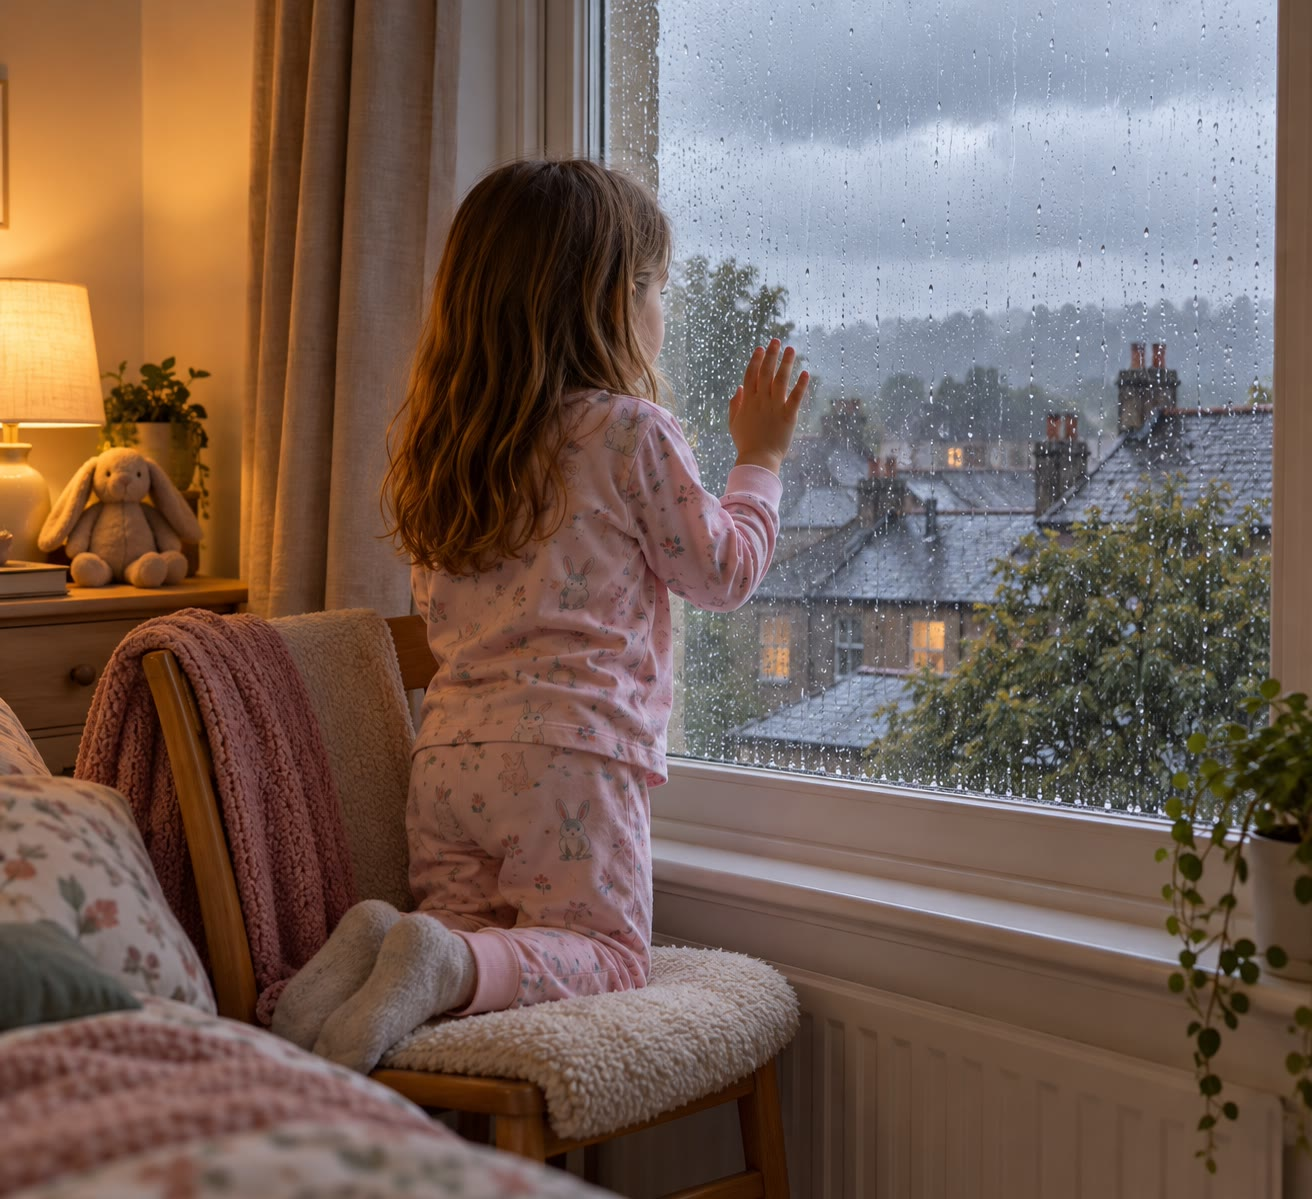
\includegraphics[width=0.72\linewidth]{images/book1/ai/g1-rainy-window.jpg}

{\small खिड़की से दिखती एक धूसर, बरसाती सुबह।}
\end{omfigure}

\begin{recall}
हर सुबह सूर्य उगता है और दिन शुरू होता है; हर शाम वह डूबता है और रात
आती है। भौतिकी की पुस्तकों में तुमने देखा है कि रात के बाद दिन क्यों
आता है। इस अध्याय में हम एक और चीज़ को देखेंगे जो हर समय बदलती रहती
है: \omterm{def:g1:watching-the-weather:weather}{मौसम}।
\end{recall}

\section{मौसम क्या है?}

जब हम बाहर जाते हैं, तो चेहरे पर हवा महसूस होती है। वह गरम हो सकती
है या ठंडी। वह थमी हुई हो सकती है, या हमारे बालों और कपड़ों को धकेल
सकती है: तब हवा चल रही होती है। हम ऊपर आसमान की ओर देखते हैं। वह नीला
और चमकीला हो सकता है, या बादलों से ढका हुआ। कभी बादलों से बारिश
गिरती है, कभी बर्फ़। यह सब मिलकर \omterm{def:g1:watching-the-weather:weather}{मौसम} है।

\begin{definition}[मौसम]\label{def:g1:watching-the-weather:weather}
किसी एक जगह पर, किसी एक पल में हवा और आसमान जैसे हैं, वही
\emph{मौसम}\index{मौसम} है: धूप वाला या बादल वाला, सूखा या बरसाती या
बर्फ़ीला, शांत या हवादार, गरम या ठंडा।
\end{definition}

\omterm{def:g1:watching-the-weather:weather}{मौसम} का वर्णन करने के लिए हम कुछ आसान सवालों के जवाब देते हैं:
\begin{enumerate}
  \item \textbf{आसमान कैसा दिखता है?} क्या वह नीला है और सूर्य चमक रहा
        है? क्या कुछ बादल हैं, या पूरा आसमान धूसर है?
  \item \textbf{क्या आसमान से कुछ गिर रहा है?} बारिश? बर्फ़? कुछ भी नहीं?
  \item \textbf{क्या हवा चल रही है?} क्या पेड़ों की पत्तियाँ हिल रही हैं?
        क्या कोई झंडा फहरा रहा है?
  \item \textbf{गरमी है या ठंड?} क्या हमें कोट चाहिए?
\end{enumerate}

\begin{omfigure}
\begin{minipage}[b]{0.49\linewidth}\centering
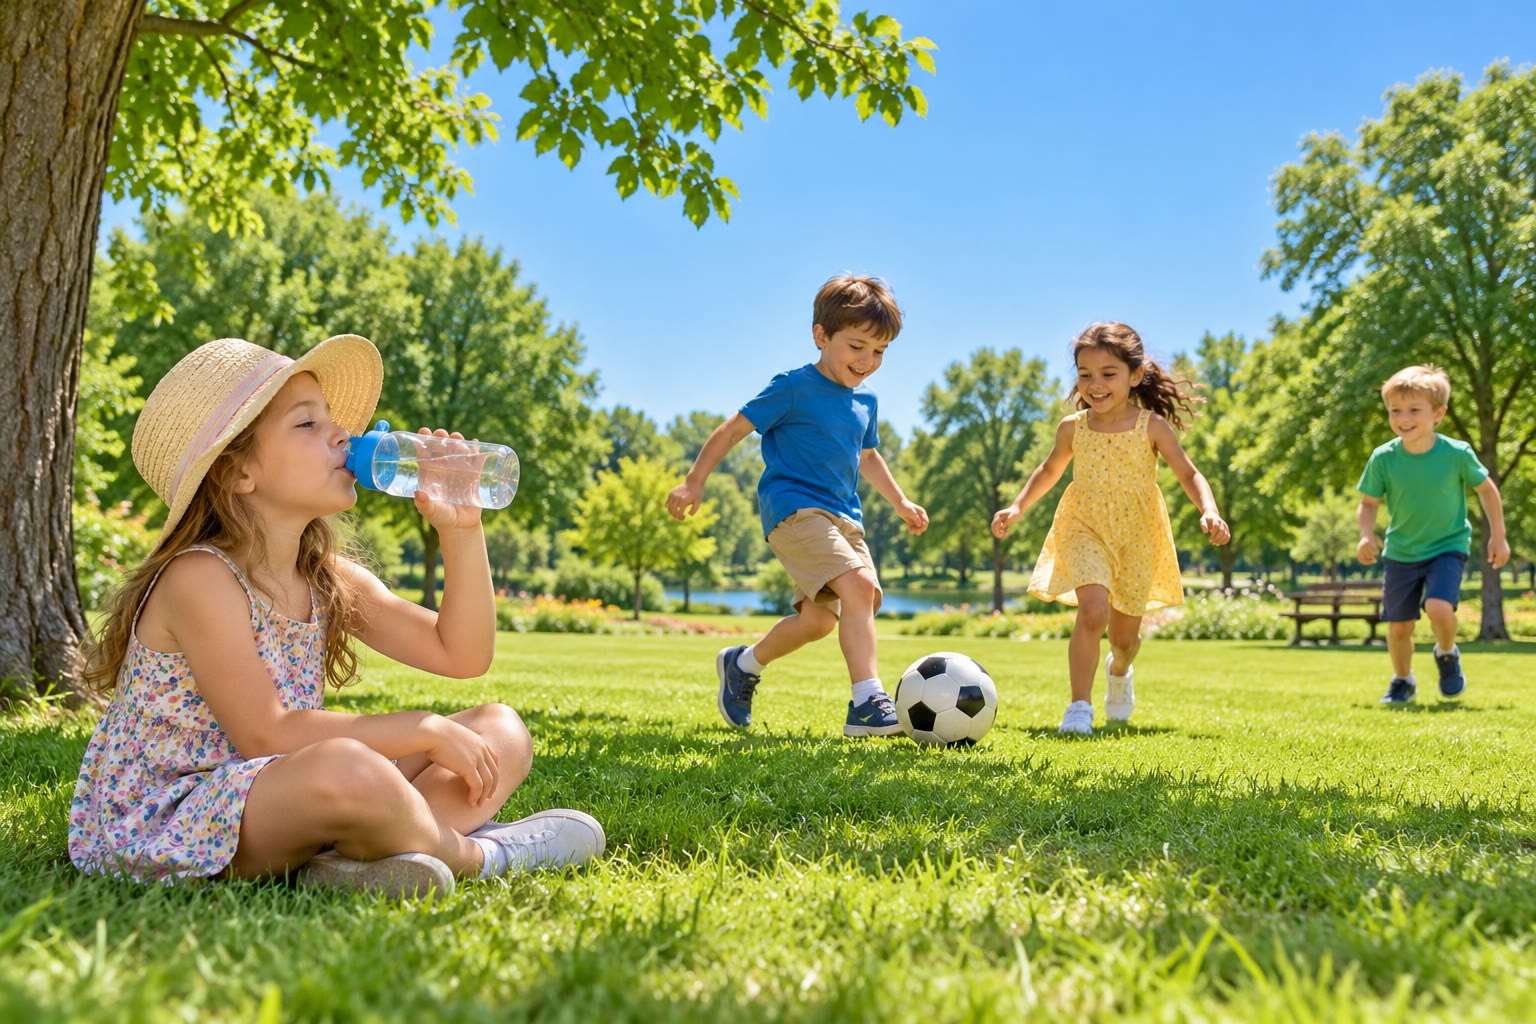
\includegraphics[width=\linewidth]{images/book1/ai/g1-sunny-park.jpg}

{\small धूप और गरमी।}
\end{minipage}\hfill
\begin{minipage}[b]{0.49\linewidth}\centering
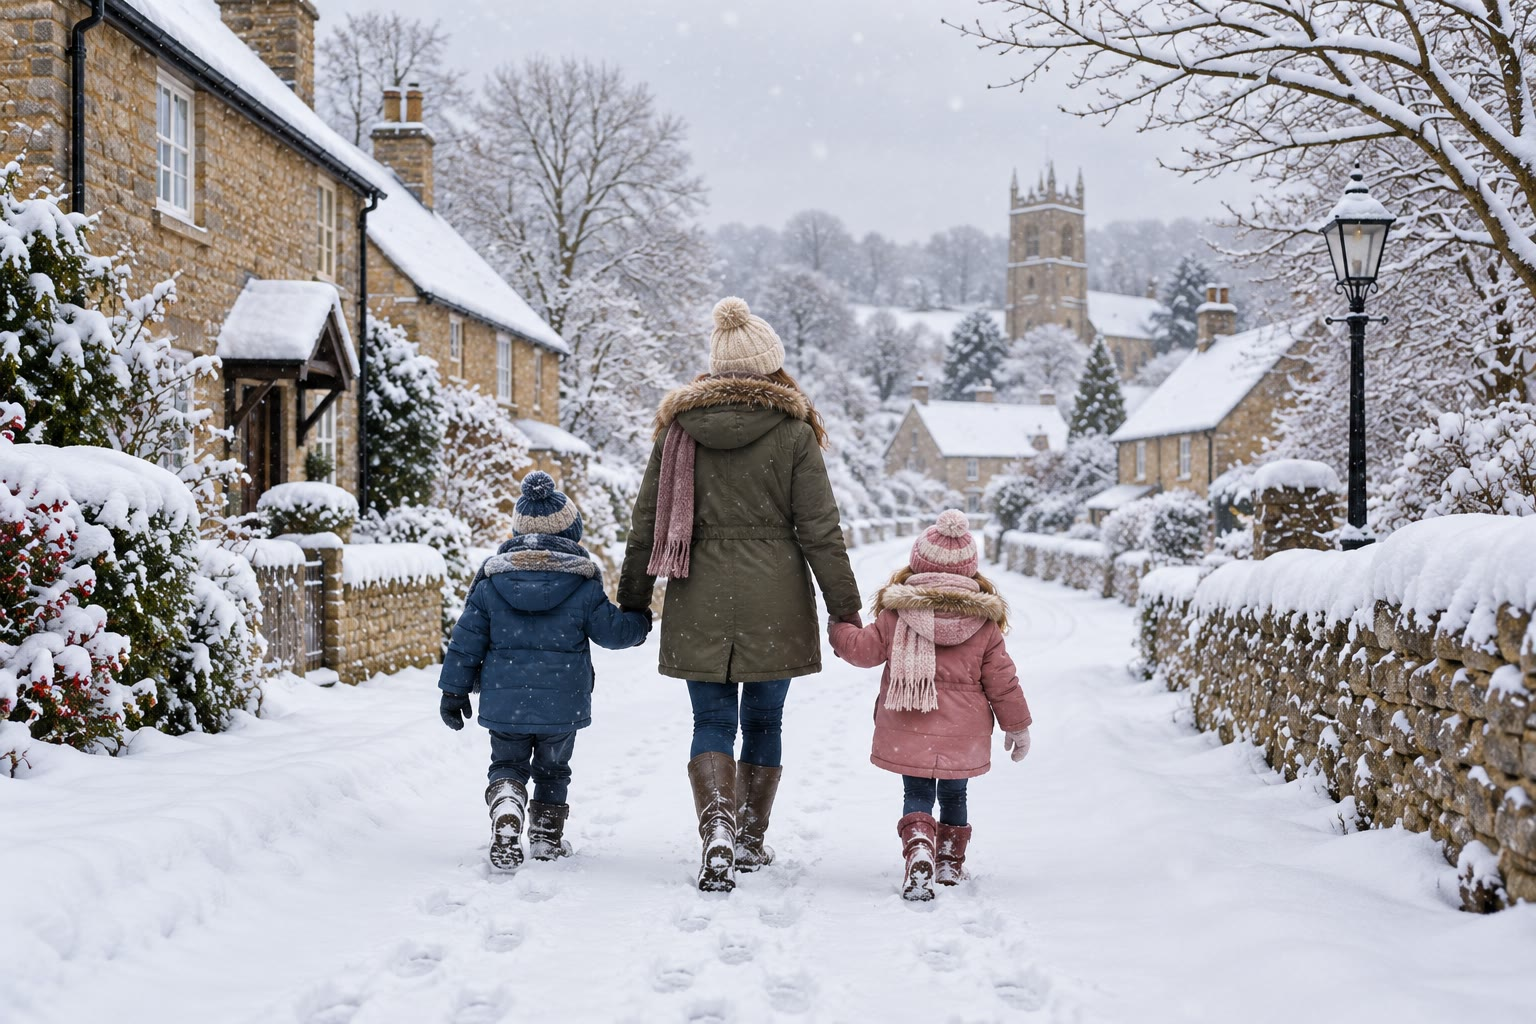
\includegraphics[width=\linewidth]{images/book1/ai/g1-snowy-street.jpg}

{\small बर्फ़ और ठंड।}
\end{minipage}

\medskip
\begin{minipage}[b]{0.49\linewidth}\centering
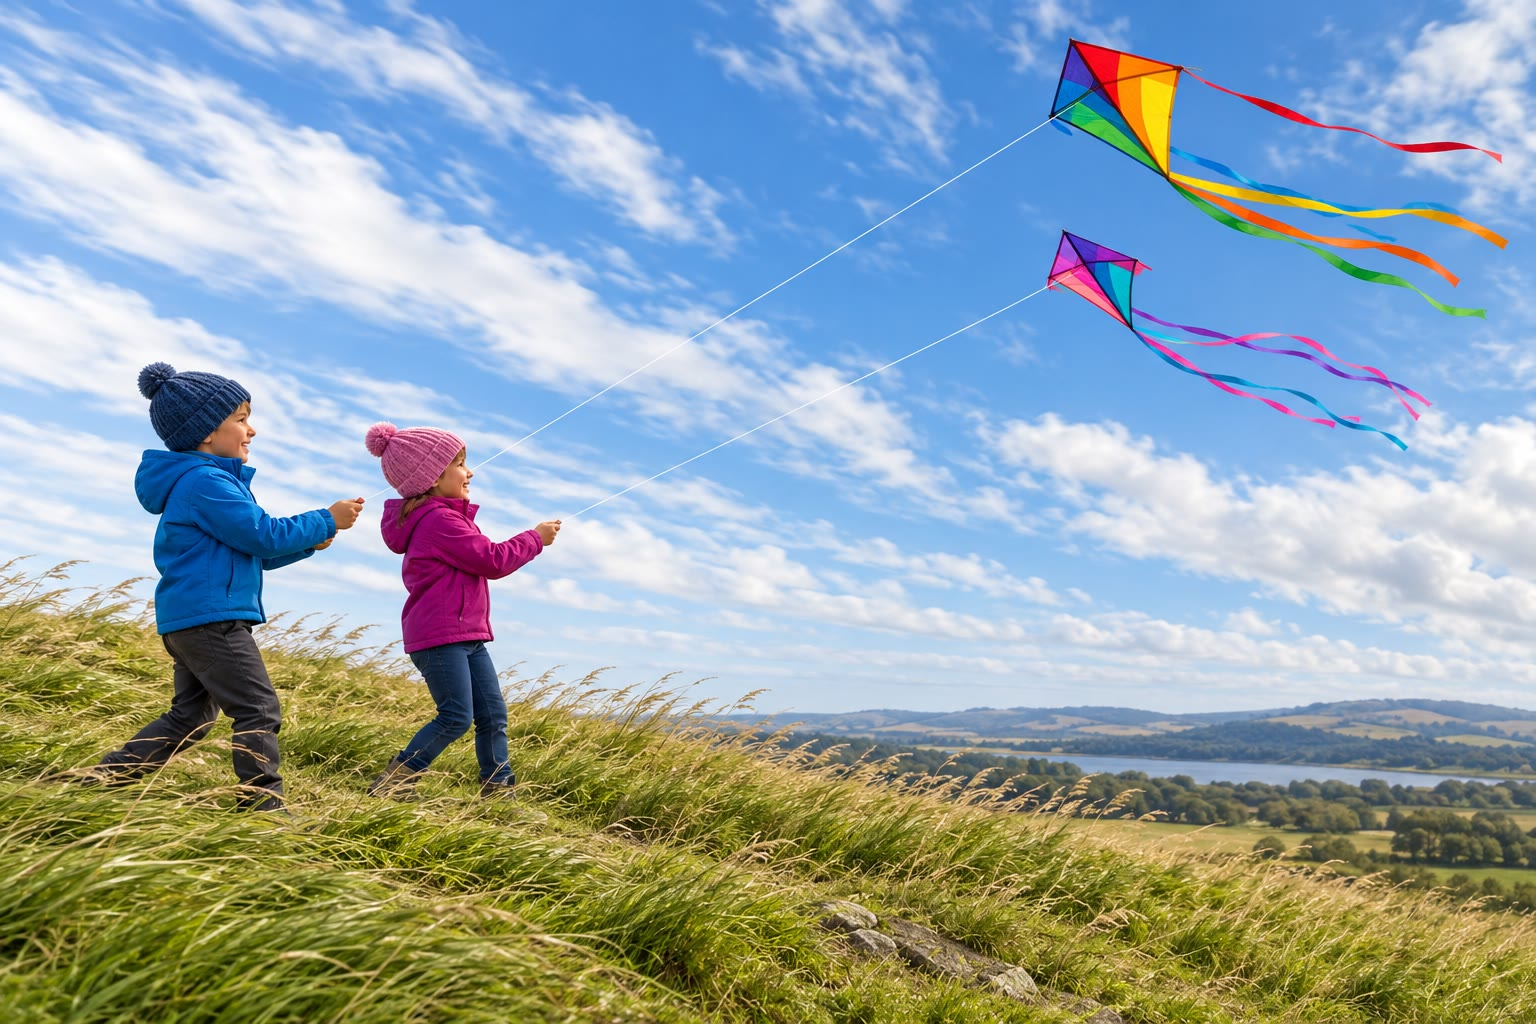
\includegraphics[width=\linewidth]{images/book1/ai/g1-windy-kites.jpg}

{\small तेज़ हवा: पतंगें उड़ रही हैं।}
\end{minipage}\hfill
\begin{minipage}[b]{0.49\linewidth}\centering
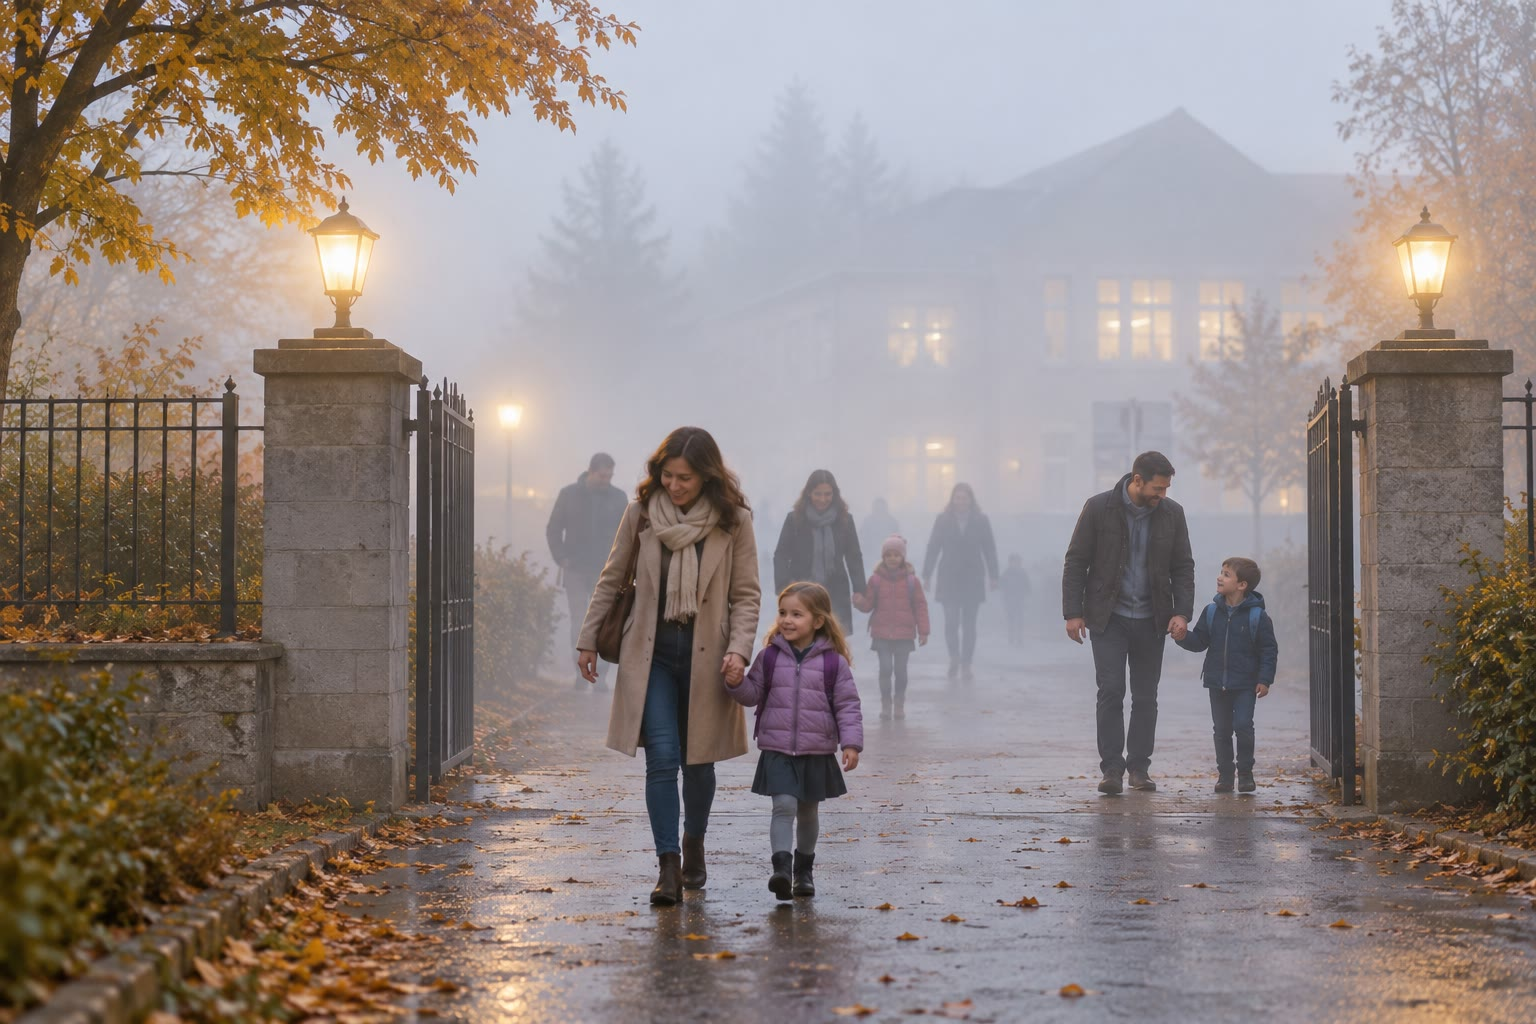
\includegraphics[width=\linewidth]{images/book1/ai/g1-foggy-school.jpg}

{\small कोहरा: हम दूर तक नहीं देख पाते।}
\end{minipage}
\end{omfigure}

\begin{example}[कोहरा]\label{ex:g1:watching-the-weather:fog}
कुछ सुबहों को हवा ख़ुद ही सफ़ेद दिखती है, और सड़क के छोर के पेड़ जैसे
ग़ायब हो जाते हैं। यह कोहरा है। कोहरा ऐसा बादल है जो ज़मीन को छूता है।
दिन गरम होने पर कोहरा अक्सर छँट जाता है।
\end{example}

\section{मौसम-चिह्न और मौसम-तालिका}

\omterm{def:g1:watching-the-weather:weather}{मौसम} को शब्दों में लिखने में बहुत समय लगता है। इसलिए \omterm{def:g1:watching-the-weather:weather}{मौसम} पर नज़र रखने
वाले लोग शब्दों की जगह छोटे-छोटे चित्र बनाते हैं: \omterm{def:g1:watching-the-weather:weather-chart}{मौसम-चिह्न}। हर चिह्न
बनाने में आसान है और पहचानने में भी।

\begin{omfigure}
\begin{tikzpicture}[x=1cm, y=1cm]
  \foreach \i/\n/\t in {0/sun/धूप, 1/suncloud/धूप और बादल,
      2/cloud/बादल, 3/rain/बारिश, 4/shower/बौछारें} {
    \pic[scale=1.25, transform shape] at (\i*2.6,0) {omwx=\n};
    \node[font=\small, align=center, text width=2.4cm] at (\i*2.6,-1.05) {\t};
  }
  \foreach \i/\n/\t in {0/snow/बर्फ़, 1/storm/आँधी-तूफ़ान, 2/fog/कोहरा,
      3/wind/तेज़ हवा} {
    \pic[scale=1.25, transform shape] at (\i*2.6+1.3,-2.6) {omwx=\n};
    \node[font=\small, align=center, text width=2.4cm] at (\i*2.6+1.3,-3.65) {\t};
  }
\end{tikzpicture}

{\small नौ \omterm{def:g1:watching-the-weather:weather-chart}{मौसम-चिह्न}। आँधी-तूफ़ान में एक काला बादल और बिजली की एक कौंध
होती है; बौछारों के बीच-बीच में धूप भी निकलती है।}
\end{omfigure}

\begin{definition}[मौसम-तालिका]\label{def:g1:watching-the-weather:weather-chart}
\emph{मौसम-चिह्न}\index{मौसम-चिह्न} एक छोटा चित्र है जो एक तरह का \omterm{def:g1:watching-the-weather:weather}{मौसम}
दिखाता है। \emph{मौसम-तालिका}\index{मौसम-तालिका} एक ऐसी सारणी है जिसमें
हम दिन-प्रतिदिन, मौसम-चिह्नों से, वह \omterm{def:g1:watching-the-weather:weather}{मौसम} लिखते हैं जो हमने देखा।
\end{definition}

एक कक्षा पूरे हफ़्ते की \omterm{def:g1:watching-the-weather:weather-chart}{मौसम-तालिका} बना सकती है। हर सुबह, और फिर हर
दोपहर, एक बच्चा बाहर देखता है और सही ख़ाने में चिह्न बनाता है। हम यह भी
लिखते हैं कि गरमी है या ठंड।

\begin{omfigure}
\begin{tikzpicture}[x=1cm, y=1cm]
  \def\cw{1.9}
  \foreach \d [count=\i from 0] in {सोमवार, मंगलवार, बुधवार, गुरुवार,
      शुक्रवार, शनिवार, रविवार}
    \node[font=\scriptsize\bfseries] at ({1.6+\i*\cw+\cw/2},0.35) {\d};
  \node[font=\scriptsize\bfseries, anchor=east] at (1.45,-0.5) {सुबह};
  \node[font=\scriptsize\bfseries, anchor=east] at (1.45,-1.5) {दोपहर};
  \node[font=\scriptsize\bfseries, anchor=east, align=right] at (1.45,-2.35) {गरमी या\\ठंड?};
  \draw[black!60] (1.6,0) rectangle ({1.6+7*\cw},-2.7);
  \foreach \i in {1,...,6}
    \draw[black!60] ({1.6+\i*\cw},0.65) -- ({1.6+\i*\cw},-2.7);
  \draw[black!60] (1.6,0.65) -- ({1.6+7*\cw},0.65);
  \draw[black!60] (1.6,0.65) -- (1.6,0);
  \draw[black!60] ({1.6+7*\cw},0.65) -- ({1.6+7*\cw},0);
  \draw[black!60] (1.6,-1) -- ({1.6+7*\cw},-1);
  \draw[black!60] (1.6,-2) -- ({1.6+7*\cw},-2);
  \foreach \i/\m/\a/\w in {0/rain/rain/ठंड, 1/cloud/suncloud/ठंड,
      2/sun/sun/गरमी, 3/sun/suncloud/गरमी, 4/suncloud/shower/गरमी,
      5/fog/sun/गरमी, 6/cloud/rain/ठंड} {
    \pic[scale=0.8, transform shape] at ({1.6+\i*\cw+\cw/2},-0.5) {omwx=\m};
    \pic[scale=0.8, transform shape] at ({1.6+\i*\cw+\cw/2},-1.5) {omwx=\a};
    \node[font=\scriptsize] at ({1.6+\i*\cw+\cw/2},-2.35) {\w};
  }
\end{tikzpicture}

{\small वसंत के एक हफ़्ते में एक कक्षा की बनाई \omterm{def:g1:watching-the-weather:weather-chart}{मौसम-तालिका}।}
\label{fig:g1:watching-the-weather:chart}
\end{omfigure}

\begin{method}[मौसम-तालिका पढ़ना]\label{met:g1:watching-the-weather:read}
\omterm{def:g1:watching-the-weather:weather-chart}{मौसम-तालिका} पढ़ने के लिए:
\begin{enumerate}
  \item जिस दिन का \omterm{def:g1:watching-the-weather:weather}{मौसम} जानना है, उसका स्तंभ ढूँढो;
  \item पंक्ति देखो: सुबह की या दोपहर की;
  \item चिह्न जो \omterm{def:g1:watching-the-weather:weather}{मौसम} दिखाता है, उसका नाम बताओ।
\end{enumerate}
कितने दिन धूप रही, यह जानने के लिए एक पंक्ति पर उँगली फिराओ और सूर्य के
चिह्न गिनो।
\end{method}

\begin{example}[कक्षा की तालिका पढ़ना]\label{ex:g1:watching-the-weather:read}
इस कक्षा की तालिका में सोमवार की सुबह बारिश थी और ठंड थी। बुधवार को
पूरे दिन धूप रही। शनिवार को सुबह के कोहरे के बाद दोपहर में धूप निकल
आई। हफ़्ते की सुबहों में कक्षा ने 2 दिन सूर्य बनाया: बुधवार और
गुरुवार को।
\end{example}

\section{मौसम बदलता है}

\omterm{def:g1:watching-the-weather:weather}{मौसम} एक जैसा नहीं रहता। वह दिन भर में बदलता है, एक दिन से अगले दिन तक
बदलता है, और साल भर में भी बदलता है।

\begin{itemize}
  \item \textbf{एक दिन के भीतर।} धूसर सुबह के बाद धूप वाली दोपहर हो सकती
        है। साफ़ नीली सुबह का अंत आँधी-तूफ़ान से हो सकता है। भोर में और
        रात को आम तौर पर दोपहर से ज़्यादा ठंडक होती है।
  \item \textbf{एक दिन से अगले दिन तक।} कक्षा की तालिका देखो: हफ़्ते के
        कोई भी दो दिन बिलकुल एक जैसे नहीं हैं।
  \item \textbf{साल भर में।} गर्मियों में दिन आम तौर पर गरम होते हैं, और
        सर्दियों में आम तौर पर ठंडे; कई जगहों पर बर्फ़ सिर्फ़ सर्दियों में
        गिरती है। ऋतुएँ हर साल लौटकर क्यों आती हैं, यह भौतिकी की
        पुस्तकें समझाती हैं।
\end{itemize}

\begin{omfigure}
\begin{tikzpicture}[x=1cm, y=1cm]
  \draw[black!50, line width=0.8pt, -{Stealth[length=2.5mm]}] (0,0) -- (12.2,0);
  \foreach \x/\n/\t/\h in {0.9/fog/भोर/ठंडक, 3.5/suncloud/सुबह/सुहावना,
      6.1/sun/दोपहर/गरमी, 8.7/storm/ढलती दोपहर/गरमी और तूफ़ान,
      11.2/suncloud/शाम/कुछ ठंडक} {
    \pic[scale=1.1, transform shape] at (\x,0.85) {omwx=\n};
    \fill[black!60] (\x,0) circle (1.5pt);
    \node[font=\scriptsize\bfseries, below] at (\x,-0.12) {\t};
    \node[font=\scriptsize, below] at (\x,-0.5) {\h};
  }
\end{tikzpicture}

{\small गर्मियों का एक दिन, सुबह से शाम तक: \omterm{def:g1:watching-the-weather:weather}{मौसम} पाँच बार बदलता
है।}
\label{fig:g1:watching-the-weather:day}
\end{omfigure}

\begin{omfigure}
\begin{tikzpicture}[x=1cm, y=1cm]
  \foreach \i/\s/\c/\g/\w/\gr in {0/वसंत/green!55!black/pink!60/suncloud/green!35,
      1/गर्मी/green!45!black/green!50!black/sun/green!35,
      2/पतझड़/orange!80!black/orange!70/rain/green!25!brown!30,
      3/सर्दी/black!55/white/snow/white} {
    \begin{scope}[shift={(\i*3.15,0)}]
      \draw[black!30, rounded corners=3pt, fill=ocBlue!6] (-1.4,-0.45) rectangle (1.4,3.05);
      \fill[\gr] (-1.4,-0.45) rectangle (1.4,0);
      \draw[black!25] (-1.4,0) -- (1.4,0);
      \fill[brown!60!black] (-0.09,0) rectangle (0.09,1.0);
      \draw[brown!60!black, line width=1.6pt] (0,0.75) -- (-0.5,1.35);
      \draw[brown!60!black, line width=1.6pt] (0,0.9) -- (0.45,1.45);
      \ifnum\i<3
        \fill[\c, opacity=0.85] (0,1.55) circle (0.72);
        \ifnum\i=0 \foreach \a in {20,80,140,200,260,320} \fill[\g] (0,1.55) ++(\a:0.45) circle (0.09); \fi
        \ifnum\i=2 \foreach \x/\y in {-0.9/0.15,0.7/0.3,0.95/0.1} \fill[\g] (\x,\y) circle (0.07); \fi
      \else
        \draw[white, line width=2.4pt] (-0.5,1.35) -- (-0.35,1.17);
        \draw[white, line width=2.4pt] (0.45,1.45) -- (0.3,1.27);
      \fi
      \pic[scale=0.8, transform shape] at (0.95,2.55) {omwx=\w};
      \node[font=\small\bfseries] at (0,-0.75) {\s};
    \end{scope}
  }
\end{tikzpicture}

{\small चारों ऋतुओं में एक ही पेड़: वसंत में फूल, गर्मी में घनी हरी
पत्तियाँ, पतझड़ में झड़ती नारंगी पत्तियाँ, सर्दी में बर्फ़ से ढकी नंगी
डालियाँ।}
\label{fig:g1:watching-the-weather:seasons}
\end{omfigure}

\begin{remark}[हवा कहाँ से आती है]\label{rem:g1:watching-the-weather:wind}
हवा हमें दिखती नहीं, पर वह जो करती है, वह हमें दिखता है। झंडे को,
हवा-थैली को या चिमनी के धुएँ को हवा धकेलती है: वे उस ओर इशारा करते हैं
जिधर हवा जा रही है, इसलिए हवा दूसरी ओर से आती है।
\end{remark}

\begin{omfigure}
\begin{tikzpicture}[x=1cm, y=1cm]
  % ground
  \fill[green!30!omLithAlluv] (-0.4,-0.1) rectangle (8.4,0);
  % windsock on a pole
  \draw[black!70, line width=1.2pt] (1,0) -- (1,3.2);
  \fill[orange!85, draw=black!60] (1,3.15) -- (3.4,2.95) -- (3.4,2.55) -- (1,2.45) -- cycle;
  \fill[white] (1.6,3.1) -- (2.2,3.05) -- (2.2,2.5) -- (1.6,2.47) -- cycle;
  \fill[white] (2.8,3.0) -- (3.4,2.95) -- (3.4,2.55) -- (2.8,2.53) -- cycle;
  \draw[black!60] (1,3.15) -- (3.4,2.95) -- (3.4,2.55) -- (1,2.45);
  % flag
  \draw[black!70, line width=1.2pt] (5.4,0) -- (5.4,3.2);
  \fill[ocBlue!70, draw=black!60] (5.4,3.15) .. controls (6.0,3.3) and (6.4,2.9) .. (7.1,3.05)
     -- (7.1,2.35) .. controls (6.4,2.2) and (6.0,2.6) .. (5.4,2.45) -- cycle;
  % wind arrows
  \foreach \y in {1.0,1.6}
    \draw[omWxRain, line width=1.4pt, -{Stealth[length=3mm]}] (-0.3,\y) -- (0.7,\y);
  \node[font=\small, align=right, anchor=east] at (-0.45,1.3) {हवा यहाँ\\से आती है};
  \draw[black!60, -{Stealth[length=2mm]}] (4.1,2.75) -- (4.9,2.75);
  \node[font=\small, align=left, anchor=west] at (7.5,2.7) {झंडा और हवा-थैली\\उधर इशारा करते हैं\\जिधर हवा जाती है};
\end{tikzpicture}

{\small तेज़ हवा वाले दिन एक हवा-थैली और एक झंडा। हवा बाएँ से दाएँ बह
रही है।}
\end{omfigure}

\section{हम मौसम पर नज़र क्यों रखते हैं?}

बहुत-से लोगों को यह जानना होता है कि \omterm{def:g1:watching-the-weather:weather}{मौसम} कैसा रहेगा।
\begin{itemize}
  \item \textbf{किसान} घास काटने से पहले आसमान देखते हैं: बारिश उसे ख़राब
        कर देगी। वसंत में उन्हें पाले वाली रात का डर रहता है, जो नन्हे
        पौधों को मार सकती है।
  \item \textbf{नाविक और मछुआरे} हवा पर नज़र रखते हैं: तेज़ हवा से ऊँची
        लहरें उठती हैं, और नावें बंदरगाह में ही रहती हैं।
  \item \textbf{विमान-चालकों} को विमान के उड़ान भरने से पहले कोहरे,
        तूफ़ानों और हवा के बारे में जानना होता है।
  \item \textbf{एक कक्षा} जो जंगल की सैर पर जा रही है, जानना चाहती है कि
        बरसाती ले जाएँ या धूप वाली टोपियाँ।
\end{itemize}
हर दिन मौसम-विज्ञानी कहलाने वाले लोग पूरी दुनिया के \omterm{def:g1:watching-the-weather:weather}{मौसम} पर नज़र रखते
हैं और रेडियो, टेलीविज़न या फ़ोन पर हमें बताते हैं कि अगले दिनों में
\omterm{def:g1:watching-the-weather:weather}{मौसम} शायद कैसा रहेगा।

\begin{example}[आसमान के संकेत]\label{ex:g1:watching-the-weather:signs}
रेडियो और फ़ोन से बहुत पहले लोगों ने आसमान को पढ़ना सीख लिया था। जब
दोपहर में छोटे सफ़ेद बादल बढ़कर ऊँची काली मीनारें बन जाते हैं, तो बौछार
या आँधी-तूफ़ान आने वाला होता है। जब हवा दिशा बदलती है और आसमान धीरे-धीरे
धूसर परदे से भर जाता है, तो अक्सर कुछ घंटों बाद बारिश होती है। ये संकेत
हमेशा सही नहीं होते, पर अक्सर काम के होते हैं।
\end{example}

\section{मौसम के हिसाब से कपड़े}

अब लीना अपने सवाल का जवाब दे सकती है। बारिश हो रही है और ठंड है, इसलिए
वह अपनी बरसाती और अपने जूते पहनेगी। कल \omterm{def:g1:watching-the-weather:weather}{मौसम} अलग हो सकता है, और वह फिर
से चुनेगी।

\begin{omfigure}
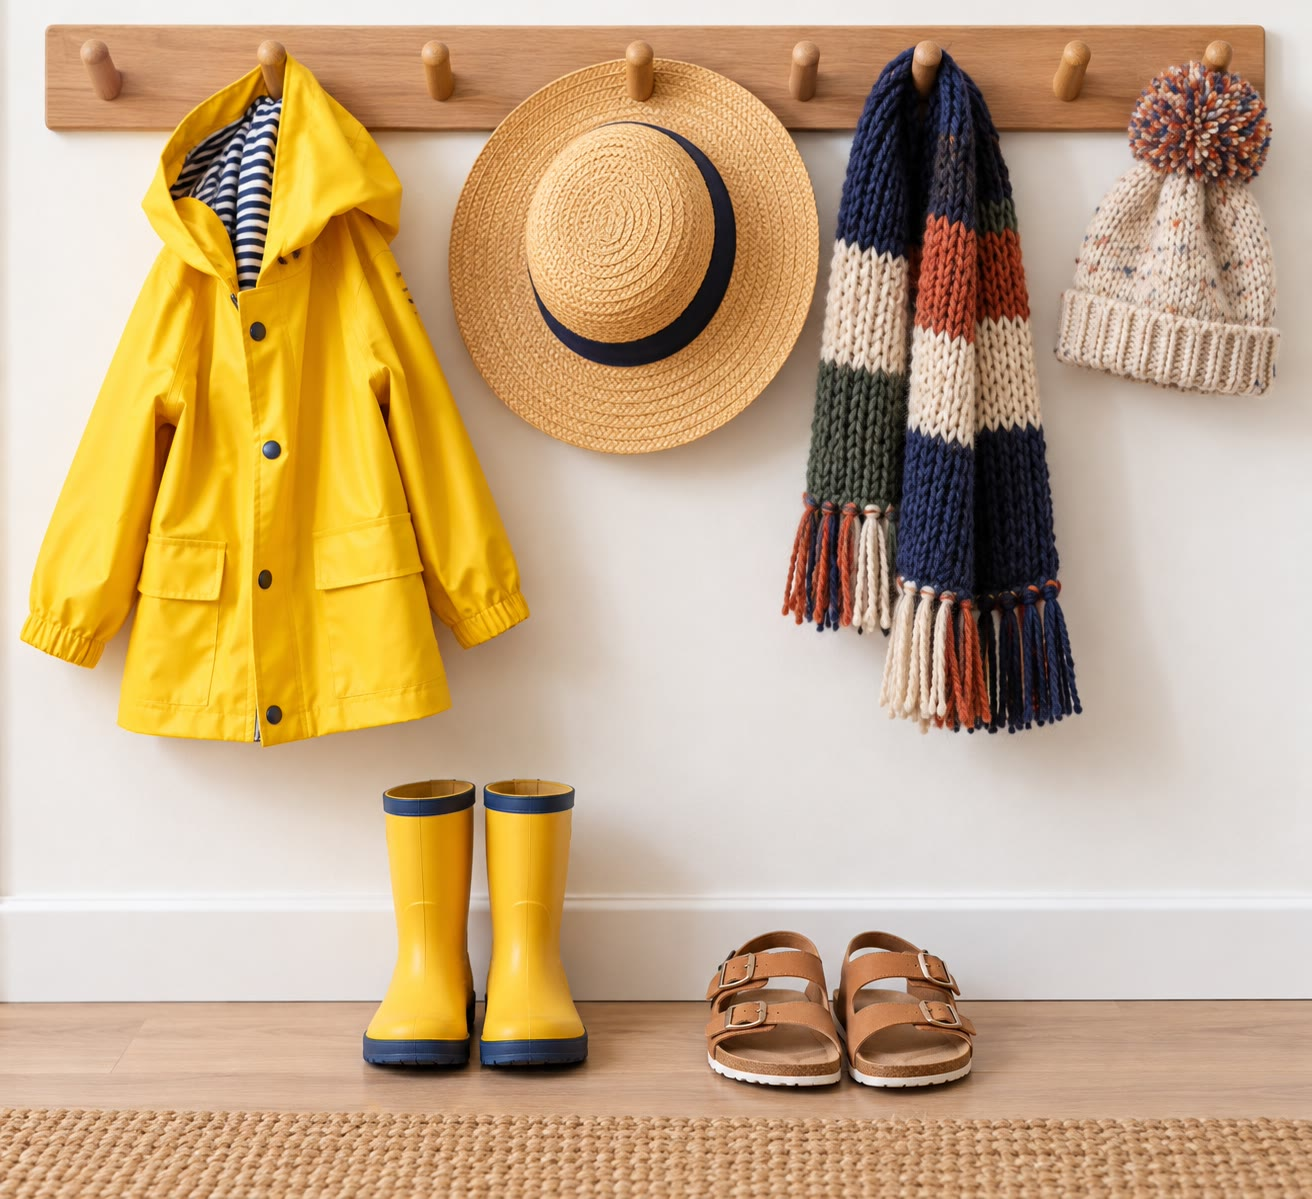
\includegraphics[width=0.66\linewidth]{images/book1/ai/g1-coat-pegs.jpg}

{\small हर तरह के \omterm{def:g1:watching-the-weather:weather}{मौसम} के कपड़े: बरसाती, धूप वाली टोपी, गुलूबंद और
गरम टोपी, लंबे जूते और सैंडल।}
\end{omfigure}

\begin{method}[मौसम के हिसाब से कपड़े चुनना]\label{met:g1:watching-the-weather:clothes}
आसमान को देखो और हवा को महसूस करो, फिर:
\begin{itemize}
  \item बारिश या बौछारें: बरसाती या छाता, और लंबे जूते;
  \item ठंड या बर्फ़: गरम कोट, गुलूबंद, टोपी और दस्ताने;
  \item तेज़ धूप और गरमी: धूप वाली टोपी, हल्के कपड़े, और पीने के लिए
        पानी;
  \item तेज़ हवा: अच्छी तरह बंद होने वाला कोट; छाता ज़्यादा काम नहीं आता।
\end{itemize}
\end{method}

\begin{safety}
\textbf{सूर्य की ओर सीधे कभी मत देखो}, एक पल के लिए भी नहीं, और चश्मे,
दूरबीन या कैमरे से तो कभी नहीं: इससे तुम्हारी आँखों को हमेशा के लिए
चोट पहुँच सकती है। जब आँधी-तूफ़ान हो, तो घर के अंदर या कार में रहो,
ऊँचे पेड़ों और पानी से दूर रहो, और तूफ़ान गुज़रने तक इंतज़ार करो।
\end{safety}

\section{अभ्यास}

\begin{exercise}[$\star$]\label{exo:g1:watching-the-weather:1}
हर तरह के \omterm{def:g1:watching-the-weather:weather}{मौसम} का चिह्न बनाओ: धूप; बारिश; बर्फ़; बादल।
\end{exercise}

\begin{exercise}[$\star$]\label{exo:g1:watching-the-weather:2}
``\omterm{def:g1:watching-the-weather:weather}{मौसम} क्या है?'' अनुभाग के चारों चित्रों में से हर एक में \omterm{def:g1:watching-the-weather:weather}{मौसम} कैसा
है? हर एक के लिए एक या दो शब्द लिखो।
\end{exercise}

\begin{exercise}[$\star$]\label{exo:g1:watching-the-weather:3}
कक्षा की \omterm{def:g1:watching-the-weather:weather-chart}{मौसम-तालिका} देखो। मंगलवार की सुबह \omterm{def:g1:watching-the-weather:weather}{मौसम} कैसा था? शुक्रवार की
दोपहर? रविवार की दोपहर?
\end{exercise}

\begin{exercise}[$\star$]\label{exo:g1:watching-the-weather:4}
कक्षा की \omterm{def:g1:watching-the-weather:weather-chart}{मौसम-तालिका} में किस दिन सुबह भी धूप थी और दोपहर में भी?
\end{exercise}

\begin{exercise}[$\star$]\label{exo:g1:watching-the-weather:5}
हर कपड़े को एक \omterm{def:g1:watching-the-weather:weather}{मौसम} से मिलाओ: धूप वाली टोपी; लंबे जूते और बरसाती;
गुलूबंद और दस्ताने। \omterm{def:g1:watching-the-weather:weather}{मौसम} ये हैं: ठंड और बर्फ़; गरमी और तेज़ धूप;
बारिश।
\end{exercise}

\begin{exercise}[$\star$]\label{exo:g1:watching-the-weather:6}
लीना कहती है: ``देखो, झंडा फहरा रहा है!'' \omterm{def:g1:watching-the-weather:weather}{मौसम} कैसा है?
\end{exercise}

\begin{exercise}[$\star$]\label{exo:g1:watching-the-weather:7}
सही या ग़लत? कारण बताओ।
\begin{enumerate}
  \item सुबह और दोपहर में \omterm{def:g1:watching-the-weather:weather}{मौसम} हमेशा एक जैसा रहता है।
  \item कोहरा ऐसा बादल है जो ज़मीन को छूता है।
  \item ``सूर्य की ओर कभी मत देखो, एक आँख से भी नहीं'' --- यह एक अच्छा नियम है।
\end{enumerate}
\end{exercise}

\begin{exercise}[$\star\star$]\label{exo:g1:watching-the-weather:8}
कक्षा की \omterm{def:g1:watching-the-weather:weather-chart}{मौसम-तालिका} में बारिश या बौछारों वाली दोपहरें गिनो। ठंडे दिन
गिनो। हफ़्ता ज़्यादातर गरम रहा या ज़्यादातर ठंडा?
\end{exercise}

\begin{exercise}[$\star\star$]\label{exo:g1:watching-the-weather:9}
सैम ने एक दिन अपनी खिड़की से यह देखा: सुबह धूसर आसमान; दोपहर के खाने
के समय खिड़की पर बूँदें; शाम को कुछ बादलों वाला नीला आसमान। तीनों
\omterm{def:g1:watching-the-weather:weather-chart}{मौसम-चिह्न} सही क्रम में बनाओ।
\end{exercise}

\begin{exercise}[$\star\star$]\label{exo:g1:watching-the-weather:10}
हवा-थैली और झंडे वाले चित्र में हवा बाईं ओर से आती है। किसी और दिन एक झंडा
बाईं ओर इशारा करता है। उस दिन हवा किस ओर से आती है?
\end{exercise}

\begin{exercise}[$\star\star$]\label{exo:g1:watching-the-weather:11}
चारों ऋतुओं वाले एक ही पेड़ का चित्र देखो। किस ऋतु में पेड़ पर पत्तियाँ
नहीं होतीं? किस ऋतु में उस पर फूल होते हैं? सर्दी के लिए कौन-सा
\omterm{def:g1:watching-the-weather:weather-chart}{मौसम-चिह्न} बना है, और वह उस ऋतु पर क्यों ठीक बैठता है?
\end{exercise}
